\documentclass[12pt,letterpaper,onecolumn]{report}
\usepackage[utf8]{inputenc}
\usepackage{amsmath}
\usepackage{amsfonts}
\usepackage{amssymb}
\usepackage{amstext}
\usepackage{amsthm}
\usepackage{graphicx}
\usepackage{exscale}
\usepackage[mathscr]{eucal}
\usepackage{bm}
\usepackage{eqlist}
\usepackage[usenames, dvipsnames]{color}
\DeclareGraphicsExtensions{.pdf, .jpg}
\newcommand{\harpoon}{\overset{\rightharpoonup}}

\usepackage{hyperref}
\usepackage{esint}
\usepackage{mathtools}
\usepackage{colortbl}
\usepackage{color}
\usepackage[utf8]{inputenc}

\usepackage[left=1in,right=1in,top=1in,bottom=1in]{geometry}

\usepackage{enumitem}
\usepackage{fancyhdr}
\pagestyle{fancy}
%\fancyhf{}
\lhead{\textbf{Lab 1}}
\chead{\textbf{ENGR 3230: Analog Circuit Design}}
\rhead{10 pts}


\begin{document}

\begin{center}
\LARGE{\textbf{Lab 1: Intro to KiCAD and PCBs}}\\
\Large{Due: Tuesday 01/29/2019}
\\

\end{center}

\section*{Objectives}
\begin{enumerate}
\item To become familiar with PCB layout and design in KiCAD
\item To build and verify a PCB

\end{enumerate}

\section*{Supplies}
\begin{itemize}
\item Computer
\item PCB Mill
\item 1 sided FR-1
\item Components
\end{itemize}

\section*{Procedure}
Your task is to design, build and verify the operation of a printed circuit board.  The circuit you are going to implement is a BJT voltage divider amplifier, shown in Figure \ref{Fig1}.  You may replace the 20 $\mu$F capacitor with a 10$\mu$F capacitor.\\

\noindent\underline{Each person will complete their PCB design individually, and make their own PCB.}

\begin{figure}[ht]
\begin{center}
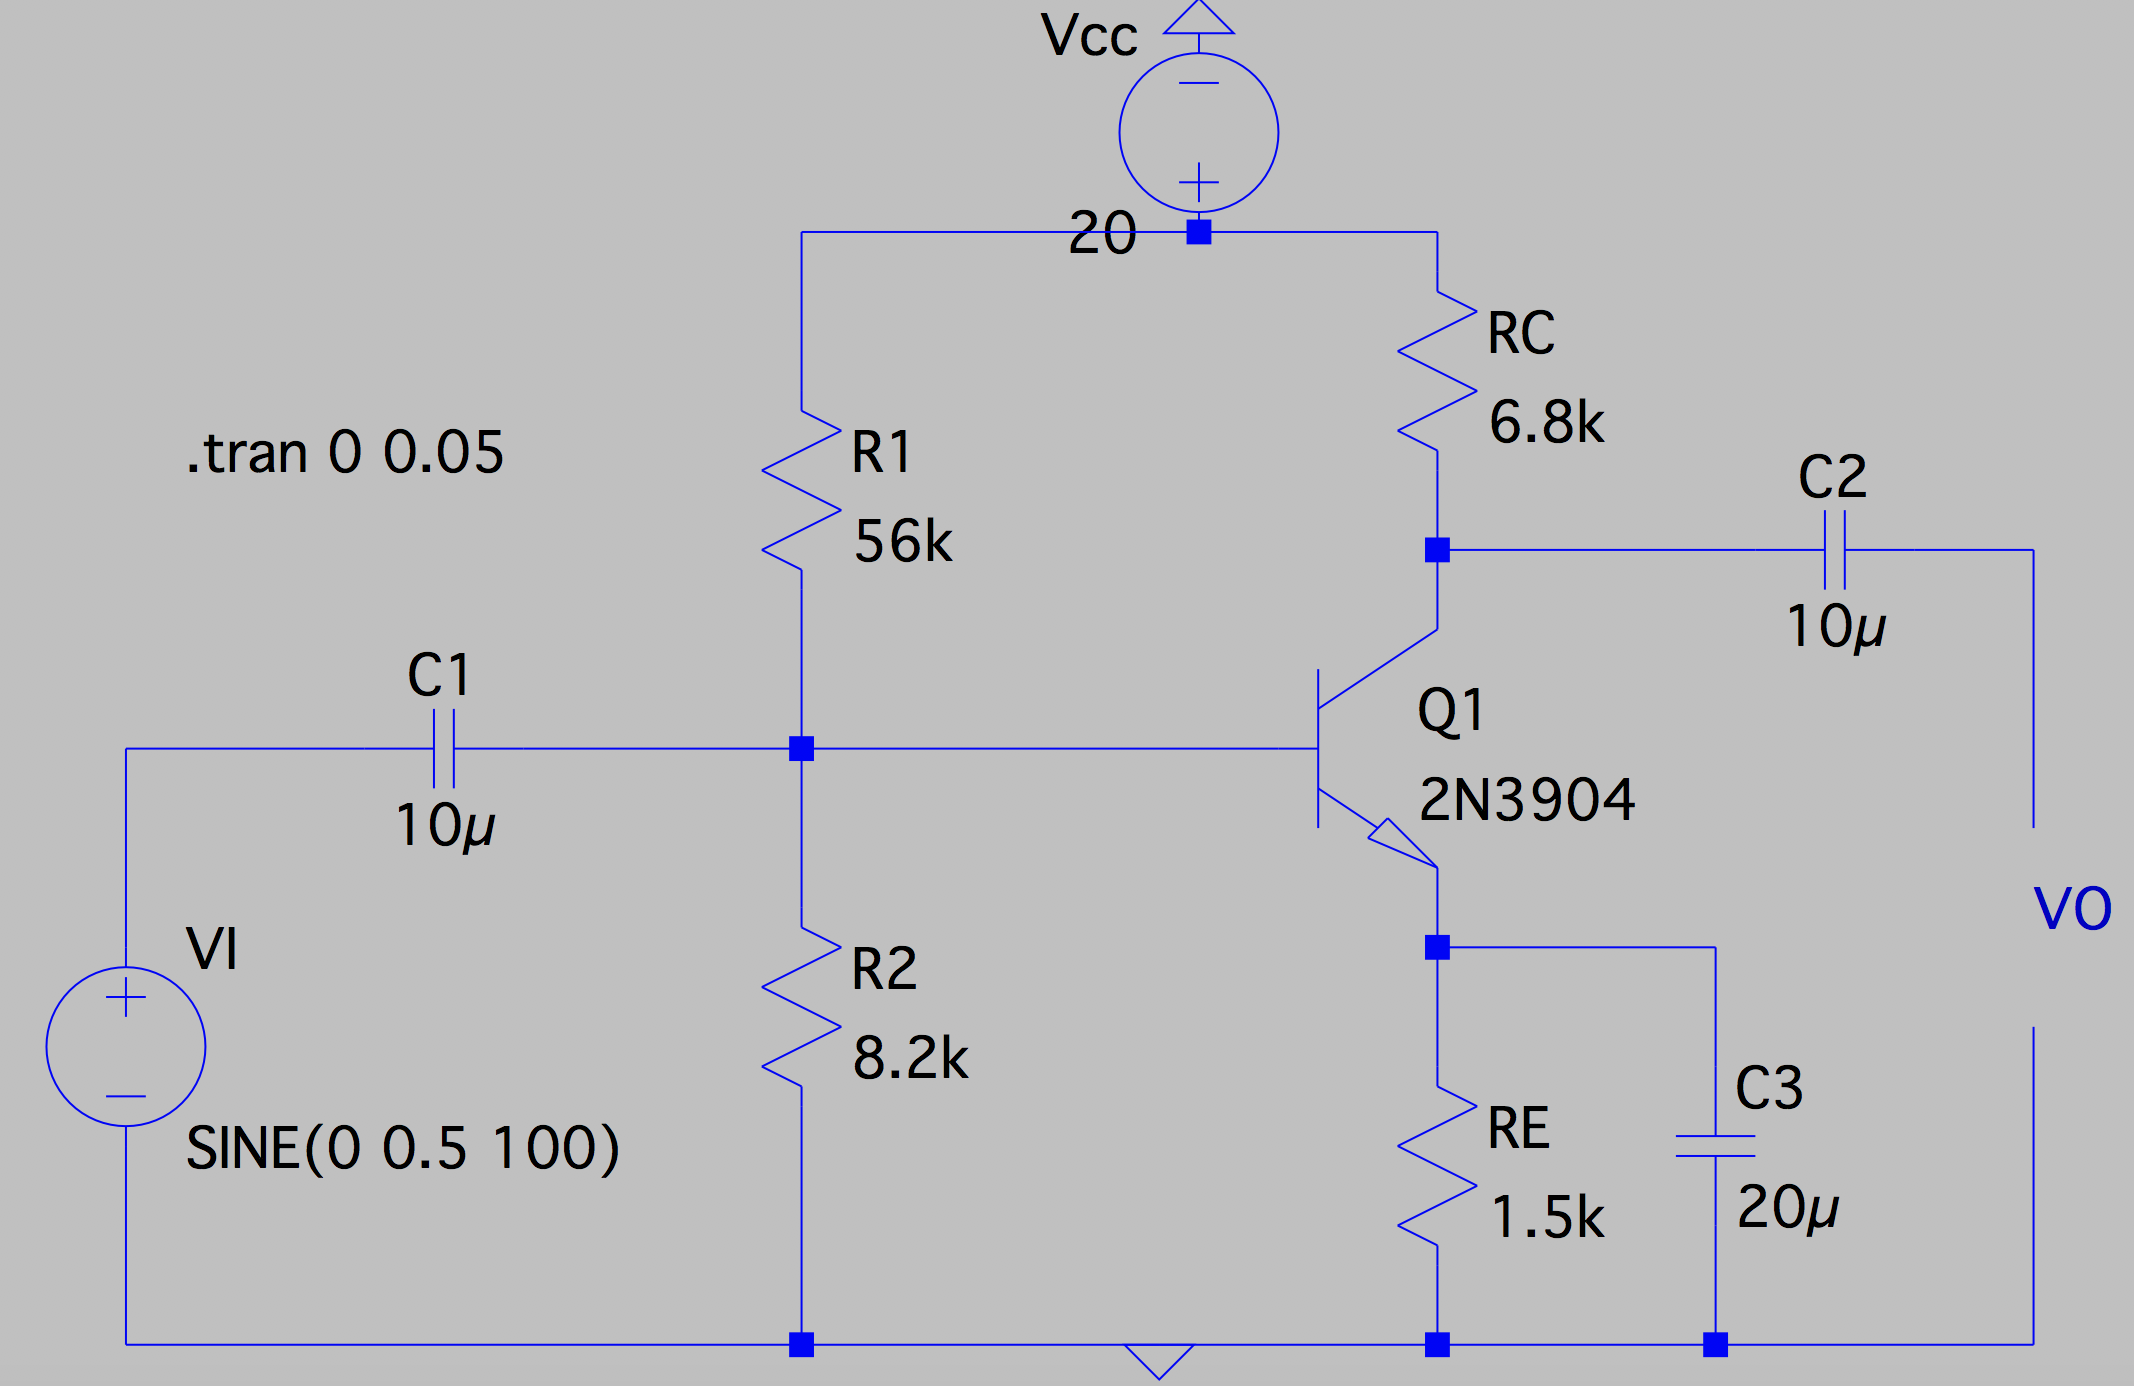
\includegraphics[width=0.75\textwidth]{Figures/VD_BJT_amp.png}
\caption{Voltage divider amplifier.}
\label{Fig1}
\end{center}
\end{figure}

\begin{enumerate}
\item Use LTSpice to simulate the circuit from Figure \ref{Fig1}.  This will be used to verify the operation of your PCB.
\item Learn how to do PCB design and layout in KiCAD using the document KiCAD\_ tutorial\_ acd\_ pcb.pdf and the video found here: \url{https://youtu.be/SpI7A8xaRJw}.
\item Make your PCB design, and generate Gerber files.
\item Use Bantam Tools to verify your Gerber files can be milled.
\item Use the OtherMill to make your PCB.
\item Populate the PCB with components, and solder them into place.
\item Using a function generator and oscilloscope, verify the operation of the amplifier.
\end{enumerate}

\section*{Requirements}
\noindent Submit each of the following on Canvas
\begin{itemize}
\item Your LTSpice file.
\item All files generated by KiCAD, including your Gerber files.
\item A screenshot of the oscilloscope verifying operation of your PCB.
\end{itemize}
\noindent In addition, please submit your populated PCB to the instructor.

\end{document}
